\documentclass[10pt,a4paper]{article}
\usepackage{cite}
\usepackage[authoryear]{natbib}     
\usepackage{geometry}
\usepackage{amsmath}
\usepackage{fullpage}
\usepackage{amsfonts}
\usepackage{breqn}
\usepackage{longtable}
\usepackage{graphicx}
\usepackage{hyperref}

\title{Dynamic General Equilibrium Model for Climate Resilient Economic Development (DGE-CRED)\\
\large{Technical Report}}
\date{April 2020}
\author{Christoph Schult and Andrej Drygalla \\ Halle Institute for Economic Research}

% define citation style
\bibliographystyle{agsm}

\begin{document}
\maketitle

\section{Introduction}
This report is a guide on how to use the spatial small open economy dynamic general equilibrium model for climate change and adaptation simulations. In general the model belongs to the class of real business cycle models, because no nominal rigidities are explicitly considered. Nevertheless, it is possible to extend the model to feature also nominal rigidities. The model structure is depicted in Figure \ref{fig:ModelStructure}.
\begin{figure}[h]
\caption{Model Structure}\label{fig:ModelStructure}
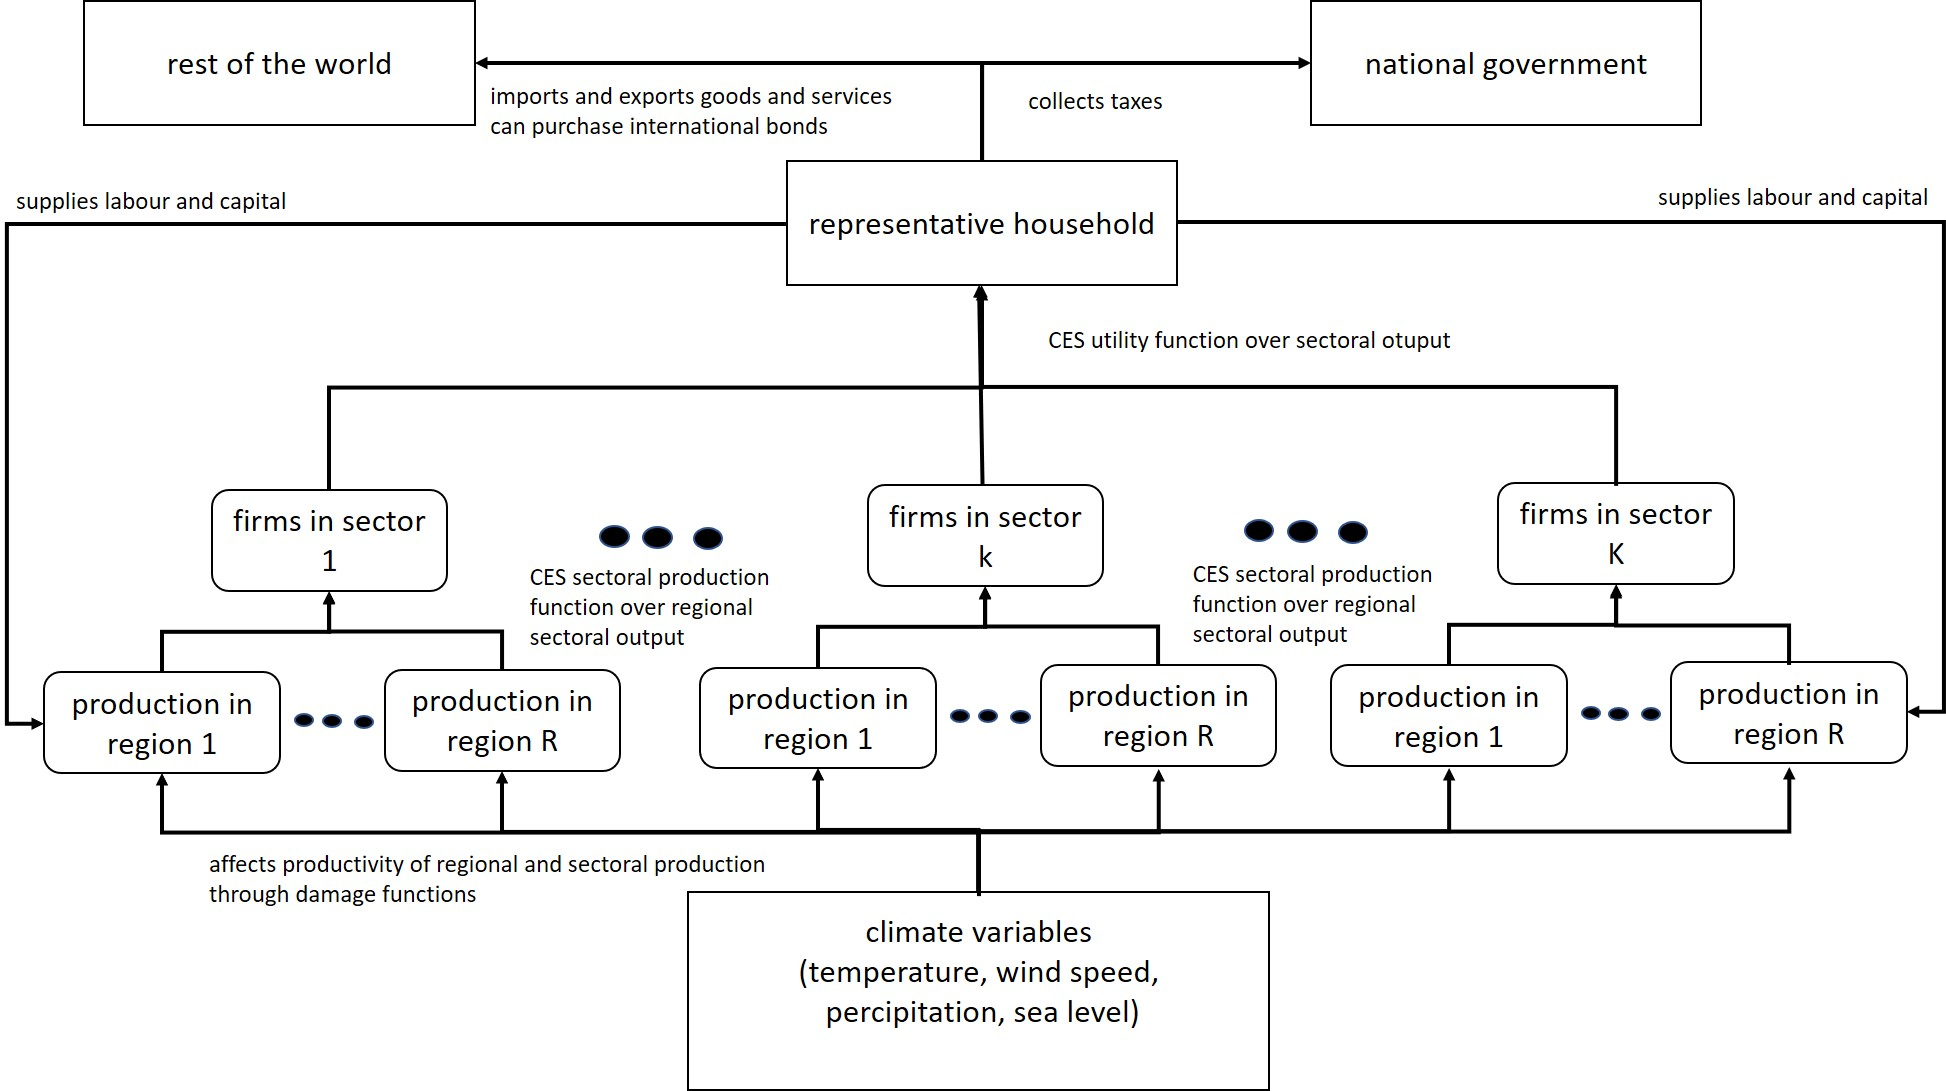
\includegraphics[width = 1\textwidth, height = 0.7\textwidth]{ModelStructure.jpg}
\end{figure}
Regional climate variables (precipitation, wind speed, temperature and sea level) are exogenous to economic variables. Regional sectoral production functions depend on regional climate variables. The model is meant to reflect small open economies and therefore the climate system is unaffected by the domestic economic system.

The model consists of an arbitrary number of regions and sectors. Regional differentiation is only provided on the supply side and not on the demand side. Representative households consume sectoral goods and supply capital and labour to the firms in the regions. Households also demand goods and services from the rest of the world. Firms use capital and labour to produce sectoral goods with sectoral and regional specific constant elasticity of substitution production functions.

The government collects taxes, consumes and can use its funds to finance adaptation measures for specific regions and sectors. So far, adaptation measures will reduce overall damage by all climate variables at the same time. The effectiveness of government expenditure in one specific region and sector can vary.

One can use the model to conduct scenario simulations to evaluate the costs and benefits for different adaptation measures. It is important to understand that the model is not meant to produce explicit forecasts for an economy. The model is meant to simulate long-run developments considering the impact of potential changes in climate variables and their effect on the supply side of the economy. the user is able to define scenarios for different climate variables and adaptation measures. Therefore, it is possible to disentangle the effect of specific climate variable changes on the economy. Further, the model is able to quantify upper limits for costs of adaptation measures to reduce damages by climate change. E.g., it is possible to evaluate the impact of temperature increases on different sectors and the overall impact on total gross value added. The discounted cumulative difference between a scenario without a temperature increase and with temperature increase can be used to determine the upper bound for the costs to reduce the damage caused by a temperature increase.  

In the following Section \ref{sec:modelderivation} the derivation of the model equations is explicitly described. Readers who are interested in using the model can skip the model section and can directly go to Section \ref{sec:modelusage}.

\cleardoublepage
\section{Model}\label{sec:modelderivation}

\subsection{Climate variables}
In order to capture the effect of climate change on the economy it is necessary to include climate variables into the model. A small open economy model does not need to include the impact of domestic economic activity on climate variables. Therefore, in contrast to \cite{nordhaus1993optimal} we do not need to model the interaction between economic activity and climate change. Climate variables are independent of other endogenous variables in the model. We explicitly model the regional average annual temperature $T_{r,t}$, the average precipitation $PREC_{r,t}$, the average annual wind speed $WS_{r,t}$, and the sea level $SL_{t}$. 
\begin{align}\label{eq:climatevariables}
T_{r,t} = T_{r,0} + \eta_{T,r,t} \nonumber \\
PREC_{r,t} = PREC_{r,0} + \eta_{PREC,r,t} \nonumber \\
W^S_{r,t} = W^S_{r,0} + \eta_{W^S,r,t} \nonumber \\
SL_{t} = SL_{0} + \eta_{SL,r,0}
\end{align}

The approach in eq.~\ref{eq:climatevariables} allows to specify the evolution of climate variables according to the projections by metreolgical models \citep[e.g.]{stocker2013climate}.

\subsection{Demand}
\subsubsection{Households}
As depicted in Figure \ref{fig:ModelStructure} the demand side is represented by representative households $h$ providing labour $N$ and capital $K$ to domestic firms $f$. Households maximize discounted utility over an infinite horizon by choosing consumption $C_t(h)$, capital $K_{k,r,t+1}(h)$, investments $I_{k,r,t}(h)$, labour $N_{k,r,t}(h)$ and foreign net bond holdings $B_{t+1}$ to maximize utility constrained by the budget constraint and the law of motion for sectoral and regional capital. Therefore, the Lagrangian eq.~\ref{eq:hhlagrangian} of the representative household is
\begin{dmath}\label{eq:hhlagrangian}
\sum_{t=0}^{\infty} \beta^{t} \left[ \left(\frac{C_{t}(h)^{1 - \sigma^{C}}}{1 - \sigma^{C}} - \sum_{k=1}^{K} \sum_{r=1}^{R} \phi^{L}_{k,r} \frac{N_{k,r,t}(h)^{1+\sigma^{L}}}{1+\sigma^{L}} \right) 
- \lambda_{t}(h) \left(P_{t} \, C_{t}(h) \, (1 + \tau^{C}) + \sum_{k=1}^{K} \sum_{r=1}^{R} P_{k,r,t} I_{k,r,t}(h) + S^{f}_{t} \, \phi^{B}_{t} \, (1 + r^{f}_{t} )\, B_{t}(h) - \sum_{k=1}^{K} \sum_{r=1}^{R} (1 - \tau^{N}) \, W_{k,r,t} N_{k,r,t}(h) - \sum_{k=1}^{K} \sum_{r=1}^{R} P_{k,r,t} \, r_{k,r,t} \, (1 - \tau^{K}) \, K_{k,r,t}(h) - B_{t+1}(h) \right) 
- \sum_{k=1}^{K} \sum_{r=1}^{R} \lambda_{t}(h) \omega^{I}_{k,r,t}(h) \left\lbrace K_{k,r,t+1} - (1 - \delta) \, K_{k,r,t} - I_{k,r,t} \, S\left(\frac{I_{k,r,t}}{I_{k,r,t-1}}\right) \right\rbrace  \right].
\end{dmath}
Households receive utility by consuming goods, where the inter temporal elasticity of consumption is defined by $\sigma^{C}$. Dis-utility from labour is sector and region specific $\phi^{L}_{k,r}$, the inverse Frisch elasticity $\sigma^{L}$ is identical for all sectors and regions. Households spent money either on consumption goods $P_t \, C_t(h) \, (1 + \tau^{C})$, regional and sector specific investment $P_{k,r,t} I_{k,r,t}(h)$ and need to repay foreign bonds $B_{t+1}(h)$. They receive income from labour $W_{k,r,t} \, N_{k,r,t}(h) \, (1 - \tau^{L})$, capital renting $P_{k,r,t} \, r_{k,r,t} \, K_{k,r,t}(h) \, (1 - \tau^{K})$ and can use their borrowed money from the foreign economy $B_{t}(h)$. The first order conditions to the problem are the behavioral equations. As is standard in teh literature we replace the Lagrange multiplier $\lambda_{t}$ by the marginal utility of consumption $\frac{C_{t}(h)^{-\sigma^{C}}}{P_{t}\, (1 + \tau^C)}$ derived from the first order condition (FOC) of the above problem with respect to (w.r.t.) consumption. Households supply labour according to the FOC w.r.t. labour eq.~\ref{eq:hhlaboursupply} for each sector and region depending on the wage $W_{k,r,t}$ and the marginal dis-utility of labour for the specific sector and region
\begin{dmath}\label{eq:hhlaboursupply}
\phi^{L}_{k,r} N_{k,r,t}(h)^{\sigma^{L}} = \lambda_{t}(h) \, W_{k,r,t} \, (1 - \tau^{N}).
\end{dmath}
The household also needs to decide how much of its income it wants to consume or invest into capital. The famous Euler equation eq.~\ref{eq:hhfoccapital} is obtained by taking the first derivative of the Lagrangian w.r.t. sector and region specific capital
\begin{dmath}\label{eq:hhfoccapital}
\lambda_{t+1}(h) \, \beta \, \left(P_{k,r,t+1} \, r_{k,r,t+1} + (1 - \delta) \, \omega^{I}_{k,r,t+1} \right) = \lambda_{t}(h) \, \omega^{I}_{k,r,t}.
\end{dmath}
Further, the household also faces investment adjustment cost $S(\frac{I_{k,r,t}}{I_{k,r,t-1}}) = 3 - exp\left\lbrace\sqrt{\phi^{K}/2}\left(\frac{I_{k,r,t}}{I_{k,r,t-1}}-1\right\rbrace\right) - exp\left\lbrace-\sqrt{\phi^{K}/2}\left(\frac{I_{k,r,t}}{I_{k,r,t-1}}-1\right)\right\rbrace$, which are sector and region specific. The specification of the investment adjustment cost function is the same as proposed and estimated by \cite{christiano2014risk} for the US.  The marginal value of sectoral and regional investment $\omega^{I}_{k,r,t}$ is determined by
\begin{dmath}\label{eq:hhfocinvestment}
P_{k,r,t} \, \lambda_{t}(h) = \lambda_{t}(h) \, \omega^{I}_{k,r,t} \, \left(S(\frac{I_{k,r,t}}{I_{k,r,t-1}}) - \frac{\partial S(\frac{I_{k,r,t}}{I_{k,r,t-1}})}{\partial I_{k,r,t}} \, \frac{I_{k,r,t}}{I_{k,r,t-1}} \right) + \beta \lambda_{t+1}(h) \, \omega^{I}_{k,r,t+1} \, \frac{\partial S(\frac{I_{k,r,t+1}}{I_{k,r,t}})}{\partial I_{k,r,t}} \, \left(\frac{I_{k,r,t+1}}{I_{k,r,t}}\right)^2
\end{dmath}
Households have access to the international financial market to purchase and sell internationally traded bonds. We only consider net foreign positions.
\begin{dmath}\label{eq:hhfocbonds}
\lambda_{t+1} \, \beta \, S^{f}_{t+1} \, \phi^{B}_{t+1} \left(1+{{r^{f}}_{t+1}}\right) = \lambda_{t} \\
\end{dmath}

The required interest rate will increase if the foreign debt relative to GDP increases and current net exports relative to GDP will decrease. 
\begin{dmath}
\phi^{B}_{t+1} = exp \left(-\phi^B \,(S^{f}_{t+1} \, r^{f}_{t+1} \, \frac{B_{t}}{Y_{t+1}}+\frac{NX_{t}}{Y_t})\right)
\end{dmath}

\subsubsection{Government}

We are interested in different policy measures taken by the government to adapt to a new climate regime. Government behavior is not a result of an optimization problem. The Government collects taxes from consumption $\tau^{C} \, C_{t}$, labour income $\sum_{k}^{K} \sum_{r}^{R} \, (\tau^{N} + \tau_{k,r,t}^{N}) \, W_{k,r,t} \, N_{k,r,t} \, PoP_{t}$ and capital income $\sum_{k}^{K} \sum_{r}^{R} \, (\tau^{K} + \tau_{r,k,t}^{K}) \, P_{k,r,t} \, r_{k,r,t} \, K_{k,r,t}$. In order to finance its activities the government can also get loans from the rest of the world $B^{G}_{t+1}$ and has to repay loans and interest from the previous period denominated in foreign currency $(1 + r^{f}_{t})$ identical to the household. The government budget constraint boils down to eq.~\ref{eq:GovBudget}.
\begin{align}\label{eq:GovBudget}
G_{t} + \sum_{k}^{K} \sum_{r}^{R} G^{A}_{k,r,t} + B^G_{t} =& \sum_{k}^{K} \sum_{r}^{R} \, \left\lbrace (\tau^{K} + \tau_{r,k,t}^{K}) \, P_{k,r,t} \, r_{k,r,t} \, K_{k,r,t} + (\tau^{N} + \tau_{k,r,t}^{N}) \, W_{k,r,t} \, N_{k,r,t} \, PoP_{t} \right\rbrace \nonumber \\
& + (1 + r^{f}_{t}) \, S^{f}_{t} \phi^{B}_{t} \, B^G_{t-1}
\end{align}

Government expenditures can be used to finance adaptation measures in specific sectors and regions $G^{A}_{k,n,t}$. Government expenditures on adaptation measures, taxes on regional and sectoral capital expenditure, and government debt are independent of other variables or to formulate it differently are discretionary. This allows us to evaluate different policy paths for the future and to model the variables by exogenous processes as stated in eq.~\ref{eq:GovExpenditure}.
\begin{align}\label{eq:GovExpenditure}
G^{A}_{k,r,t} = G^{A}_{k,r,0} + \eta^{A}_{k,r,t} \nonumber \\
\tau^{K}_{k,r,t} = \tau^{K}_{k,r,0} + \eta^{\tau^{K}}_{k,r,t} \nonumber \\
\tau^{N}_{k,r,t} = \tau^{N}_{k,r,0} + \eta^{\tau^{N}}_{k,r,t} \nonumber \\
B^G_{t} = B^G_{0} + \eta^{B^{G}}_{t}
\end{align} 


\subsubsection{Resource constraint}

Households and the Government use domestic final goods $Y_t$ produced by firms for consumption, investment and for exports $X_{t}$ and can also use imports $M_t$ for consumption and investment. This gives rise to the well known resource constraint or the expenditure approach to define GDP 
\begin{align}
Y_{t} = C_{t} + I_{t} + G_{t} + \underbrace{X_{t} - M_{t}}_{NX_{t}}
\end{align}

\subsection{Production}

Households demand final domestic goods $Y_{t}$ combining goods from different sectors $Y_{k,t}$ using a CES composition function. They minimize expenditures subject to the composition function
\begin{align}
\underset{Y_{k,t}}{\mathrm{min}} & \sum_{k} Y_{k,t} \, P_{k,t} \\ 
Y_{t} &= \left(\sum_{k} {\omega^{Q}_{k}}^{\frac{1}{\eta^Q}} Y_{k,t}^{\frac{\eta^Q-1}{\eta^Q}} \right)^{\frac{\eta^Q}{\eta^Q-1}}
\end{align}

Therefore demand for sectoral products correspond to the first order conditions of the above optimization problem. The Lagrange multiplier is the price level $P_{t}$ of domestic products. 
\begin{align}
\frac{P_{k,t}}{P_{t}} &= {\omega^{Q}_{k}}^{\frac{1}{\eta^Q}} \left(\frac{Y_{k,t}}{Y_{t}}\right)^{\frac{-1}{\eta^Q}}
\end{align}

In order to model regional economic activity we further decompose the production process on a regional level. One can either think about this approach as modeling the optimization problem of a representative firm operating in one sector on a national level allocating production activity across the nation. Another way is to consider that households make direct purchases from regional operating firms in one sector. In this case the following optimization problem would be part of the above optimization problem. 
\begin{align}
\underset{Y_{k,r,t}}{\mathrm{min}} & \sum_{k} Y_{k,r,t} \, P_{k,r,t} \\ 
Y_{k,t} &= \left(\sum_{k} {\omega^{Q}_{k,r}}^{\frac{1}{\eta^Q_{k}}} Y_{k,r,t}^{\frac{\eta^Q_{k}-1}{\eta^Q_{k}}} \right)^{\frac{\eta^Q_{k}}{\eta^Q_{k}-1}}
\end{align}

Demand for sectoral and regional products correspond to the first order conditions of the above optimization problem. The Lagrange multiplier is the sectoral price level $P_{k,t}$ of domestic products. 
\begin{align}
\frac{P_{k,r,t}}{P_{k,t}} &= {\omega^{Q}_{k,r}}^{\frac{1}{\eta^{Q}_{k}}} \left(\frac{Y_{k,r,t}}{Y_{k,t}}\right)^{\frac{-1}{\eta^{Q}_{k}}}
\end{align}

At the regional and sectoral level are representative firms maximizing profits using capital $K_{k,r,t}$ and labour $L_{k,r,t} = N_{k,r,t} \, PoP_{t}$ provided by households to produce products. They charge a price $P_{k,r,t}$ for their products and have to pay households wages $W_{k,r,t}$, interest on rented capital $P_{r,k,t} \, r_{r,k,t}$, taxes related to the wage bill $\tau^{N}_{r,k,t}$ and on capital expenditure $\tau^{K}_{r,k,t}$.  Representative firms have access to a regional and sector specific constatn elasticity of substitution production function. The productivity of capital and labour of a firm in one sector and region depends on the climate variables, and the adaption measures by the government represented by a damage function $D_{k,r,t} = D_{k,r}\left(T_{r,t}, \, PREC_{r,t}, \, W^{S}_{r,t}, \, SL_{r,t} \, G^{A}_{r,k,t} \right)$ and the exogenous level of productivity $A_{k,r,t}$. As in \cite{nordhaus1993optimal} we assume a polynomial functional form of the damage functions, but the damages are different across regions and sectors eq.~\ref{eq:Damages}.
\begin{align}\label{eq:Damages}
{{D_{k,r}}_{t}}=& exp\left(-\phi^{G^{A}_{k,r}} \, G^{A}_{k,r,t}\right) \, \Big( \nonumber \\
&\underbrace{{{a_{T,1,k,r}}} \, {{T_{r}}_{t}}+{{a_{T,2,k,r}}}\, \left({T_{r}}_{t}\right)^{a_{T,3,k,r}}}_{\mbox{impact of temperature}}+ \underbrace{{{a_{SL,1,k,r}}}\, {{SL}_{t}}+{{a_{SL,2,k,r}}}\, \left({SL}_{t}\right)^{{{a_{SL,3,k,r}}}}}_{\mbox{impact of sea level}} \nonumber \\
+ & \underbrace{{{a_{W^{S},1,k,r}}}\, {{W_{r}^{S}}_{t}}+{{a_{W^{S},2,k,r}}}\, \left({W_{r}^{S}}_{t}\right)^{{{a_{W^{S},3,k,r}}}}}_{\mbox{impact of wind speed}}
+ \underbrace{{{a_{PREC,1,k,r}}} \, {{PREC_{r}}_{t}}+{{a_{PREC,2,k,r}}}\, \left({PREC_{r}}_{t}\right)^{{{a_{PREC,3,k,r}}}}}_{\mbox{impact of precipitation}} \nonumber \\
&\Big). 
\end{align}

Firms in each region and sector have access to a constant elasticity of substitution production function with production factors labour and capital. Eq.~\ref{eq:profitoptim} states the optimization problem of the firm.
\begin{align}\label{eq:profitoptim}
\underset{Y_{k,r,t}, N_{k,r,t}, K_{k,r,t}}{\mathrm{max}} P_{k,r,t} \, Y_{k,r,t} - W_{k,r,t} \, N_{k,r,t} \, PoP_{t} - r_{k,r,t} P_{k,r,t} K_{k,r,t} \nonumber \\ 
\mbox{s.t.} \, Y_{k,r,t} = A_{k,r,t} (1 - D_{k,r,t}) \, \left[{\alpha^{N}_{k,r}}^{\frac{1}{\eta^{NK}_{k,r}}} \, \left( PoP_{t} \, N_{k,r,t}\right)^{\rho_{k,r}} + {\alpha^{K}_{k,r}}^{\frac{1}{\eta^{NK}_{k,r}}} \, \left(K_{k,r,t}\right)^{\rho_{k,r}}\right]^{\frac{1}{\rho_{k,r}}}, \nonumber \\
\mbox{ where } \rho_{k,r} = \frac{\eta^{NK}_{k} - 1}{\eta^{NK}_{k}}.
\end{align}

Demand for production factors are given by the first order condition of the above optimization problem. The Lagrange multiplier is equal to the price charged by companies. 

\begin{align}\label{eq:focfirm}
\frac{W_{k,r,t}}{P_{k,r,t}} = {\alpha^{N}_{k,r}}^{\frac{1}{\eta^{NK}_{k,r}}} \, \left(\frac{PoP_{t} N_{k,r,t}}{Y_{k,r,t}}\right)^{-\frac{1}{\eta^{NK}_{k,r}}} \nonumber \\ 
r_{k,r,t} = {\alpha^{K}_{k,r}}^{\frac{1}{\eta^{NK}_{k,r}}} \, \left(\frac{K_{k,r,t}}{Y_{k,r,t}} \right)^{-\frac{1}{\eta^{NK}_{k,r}}} \\ 
\end{align}

We use the more general case of the CES production function rather than the more commonly used Cobb-Douglas production function. The parameter $\eta^{NK}_{k,r}$ allows us to control the response of capital and labour demand to temporary productivity shocks. Temporary productivity shocks are in our set-up also weather extremes. We will discuss the problem later. 

\subsection{Rest of the world}

The demand for domestic exports and foreign imports is not explicitly modeled in this version of the model. We assume that net exports follow an auto-regressive process of order one and that the long run value of net exports depend on the long-run development of gross domestic product. We therefore assume that imports and exports will grow at the same speed as GDP. Sluggish adjusmtents in export and import behavior of companies is captured by an auto-regressive process. 
\begin{align}
NX_{t} = \rho^{NX} \, NX_{t-1} + (1 - \rho^{NX}) \omega^{NX} P_{t} \, Y_{t}
\end{align}

The effective exchange rate $S^f_{t}$ and the world interest rate $r^{f}_{t}$ determine how much governments and households have to pay back in domestic currency as net lender or how much they receive as net borrower to the rest of the world. Here the world interest rate is independent of domestic developments and only the effective exchange rate adjusts according to eq.~\ref{eq:hhfocbonds}.

\section{Scenario Analysis}





\cleardoublepage
\section{How to use the model?}\label{sec:modelusage}
\subsection{Usage}
\begin{enumerate}
\item In order to use the model you need to install \href{https://www.dynare.org/download/}{Dynare (at least version 4.6.1)}  and \href{https://www.mathworks.com/products/matlab.html}{Matlab (at least 2018b)} or \href{https://www.gnu.org/software/octave/}{Octave} on your computing machine. 
For Octave you need to have the version 5.2.0 as reported by the Dynare team. 
\item You need to download the repository from Github. 
\item Open Octave or Matlab GUI and browse to the location of the folder in your computer. You have the right folder if the command {\tt pwd()} returns {\tt YourPath/DGE-CRED/DGE_CRED_Model}.
\item The script {\tt RunSimulations.m} has to be executed in order to run simulations for different scenarios. Make sure that the scenarios and model parameters are defined in the file \\ {\tt ModelSimulationandCalibrationKSectorsandRRegions.xlsx}. We need to adopt the number of sectors and regions in the file {\tt DGE\_CRED\_Model.mod}.
\item The simulation results are stored in the file {\tt ResultsScenariosKSectorsandRRegions.xlsx}.
\end{enumerate}

\section{Folder structure}
\begin{enumerate}
\item The main file containing all necessary mod files is {\tt DGE_CRED_Model.mod}. This file includes the following files stored in the {\tt ModFiles} folder:
\begin{enumerate}
\item {\tt DGE_CRED_Model_Declarations.mod} declares all endogenous and exogenous variables if the model and structural parameters.
\item {\tt DGE_CRED_Model_Parameters.mod} assigns values to the structural parameters of the model.
\item {\tt DGE_CRED_Model_Equations.mod} contains the equations of the model.
\item {\tt DGE_CRED_Model_LatexOutput.mod} produces latex output for documentation of the declared variables and model equations.
\item {\tt DGE_CRED_Model_SteadyState.mod} computes initial and terminal condition for the dynamic simulation.
\item {\tt DGE_CRED_Model_Simulations.mod} starts the dynamic simulation.
\end{enumerate}
\item Subroutines responsible for finding the initial and terminal conditions are located in the subfolder {\tt Functions}:
\begin{enumerate}
\item {\tt Calibration.mat} finds the initial conditions to reflect a specific year of the economy.
\item {\tt FindA.mat} looks for exogenous productivity shocks across sectors and regions to meet the terminal conditions.
\item {\tt FindK.mat} looks for a capital allocation across sectors and regions to fulfill the static equations of the model.
\item {\tt rng.mat} random number generator function necessary for Octave users.
\item {\tt LoadExogenous.mat} reads exogenous variables for different scenarios.
\end{enumerate}
\item To define scenarios and structural parameters one needs to create an Excel workbook located in the subfolder {\tt ExcelFiles}:
\begin{enumerate}
\item {\tt ModelSimulationandCalibrationforKSectorsandRregions.xlsx} has multiple sheets:
\begin{enumerate}
\item initial {\tt Start}
\item terminal {\tt Terminal}
\item parameters to define rigidity parameters {\tt Dynamics}
\item elasticity parameters and tax rates {\tt Structural Parameters}
\item coefficients for regional and sector specific damage functions {\tt Climate Damage Functions}
\item {\tt Baseline} scenario and other optional scenario sheets defining paths for exogenous varibales
\end{enumerate}
\item {\tt ResultsScenariosKSectorsandRregions.xlsx} has as many sheets as Scenarios defined in the previous Excel file.
\end{enumerate}
\item The latex files produced by {\tt DGE_CRED_Model_LatexOutput.mod} are stored in {\tt LatexFiles}.
\begin{enumerate}
\item the system of dynamic equations as implemented in Matlab {\tt DGE_CRED_Model_Dynamic}, {\tt DGE_CRED_Model_Dynamic_content}
\item names of endogenous, exogenous variables and parameters {\tt DGE_CRED_Model_latex_definitions}
\item the system of dynamic equations in original form without auxiliary variables for leads and lags {\tt DGE_CRED_Model_original}, {\tt DGE_CRED_Model_original_content}
\end{enumerate}
\item The file to run different simulations is {\tt RunSimulations.m}.
\item A Matlab function to find solutions to the static system of equations is {\tt DGE_CRED_Model_steady_state.m}.
\end{enumerate}

\bibliography{references}

\appendix
\section{Model Equations}
\footnotesize
% Equation 1
\subsection{Regional Industries}
% Equation 1
damage function TFP
\begin{dmath}
{{D_{k,r}}_{t}}=exp\left(-\phi^{G^{A}_{k,r}} \, G^{A}_{k,r,t}\right) \, \left({{a_{T,1,k,r}}} \, {{T_{r}}_{t}}+{{a_{T,2,k,r}}}\, \left({T_{r}}_{t}\right)^{a_{T,3,k,r}}+{{a_{SL,1,k,r}}}\, {{SL}_{t}}+{{a_{SL,2,k,r}}}\, \left({SL}_{t}\right)^{{{a_{SL,3,k,r}}}}+{{a_{W,1,k,r}}}\, {{W_{r}^{S}}_{t}}+{{a_{W,2,k,r}}}\, \left({W_{r}^{S}}_{t}\right)^{{{a_{W,3,k,r}}}}+{{a_{P,1,k,r}}}\, {{PREC_{r}}_{t}}+{{a_{P,2,k,r}}}\, \left({PREC_{r}}_{t}\right)^{{{a_{P,3,k,r}}}}+{{a_{C,1,k,r}}}\, {{CYC_{r}}_{t}}+{{a_{C,2,k,r}}}\, \left({CYC_{r}}_{t}\right)^{{{a_{C,3,k,r}}}}+{{a_{D,1,k,r}}}\, {{DRO_{r}}_{t}}+{{a_{D,2,k,r}}}\, \left({DRO_{r}}_{t}\right)^{{{a_{DRO,3,k,r}}}}\right) 
\end{dmath}
damage function capital
\begin{dmath}
{{D^{K}_{k,r}}_{t}}=exp\left(-\phi^{G^{A}_{k,r}} \, G^{A}_{k,r,t}\right) \, \left({{a^{K}_{T,1,k,r}}} \, {{T_{r}}_{t}}+{{a^{K}_{T,2,k,r}}}\, \left({T_{r}}_{t}\right)^{a^{K}_{T,3,k,r}}+{{a^{K}_{SL,1,k,r}}}\, {{SL}_{t}}+{{a^{K}_{SL,2,k,r}}}\, \left({SL}_{t}\right)^{{{a^{K}_{SL,3,k,r}}}}+{{a^{K}_{W,1,k,r}}}\, {{W_{r}^{S}}_{t}}+{{a^{K}_{W,2,k,r}}}\, \left({W_{r}^{S}}_{t}\right)^{{{a^{K}_{W,3,k,r}}}}+{{a^{K}_{P,1,k,r}}}\, {{PREC_{r}}_{t}}+{{a^{K}_{P,2,k,r}}}\, \left({PREC_{r}}_{t}\right)^{{{a^{K}_{P,3,k,r}}}}+{{a^{K}_{C,1,k,r}}}\, {{CYC_{r}}_{t}}+{{a^{K}_{C,2,k,r}}}\, \left({CYC_{r}}_{t}\right)^{{{a^{K}_{C,3,k,r}}}}+{{a^{K}_{D,1,k,r}}}\, {{DRO_{r}}_{t}}+{{a^{K}_{D,2,k,r}}}\, \left({DRO_{r}}_{t}\right)^{{{a^{K}_{DRO,3,k,r}}}}\right) 
\end{dmath}
damage function labour productivity
\begin{dmath}
{{D^{N}_{k,r}}_{t}}=exp\left(-\phi^{G^{A}_{k,r}} \, G^{A}_{k,r,t}\right) \, \left({{a^{N}_{T,1,k,r}}} \, {{T_{r}}_{t}}+{{a^{N}_{T,2,k,r}}}\, \left({T_{r}}_{t}\right)^{a^{N}_{T,3,k,r}}+{{a^{N}_{SL,1,k,r}}}\, {{SL}_{t}}+{{a^{N}_{SL,2,k,r}}}\, \left({SL}_{t}\right)^{{{a^{N}_{SL,3,k,r}}}}+{{a^{N}_{W,1,k,r}}}\, {{W_{r}^{S}}_{t}}+{{a^{N}_{W,2,k,r}}}\, \left({W_{r}^{S}}_{t}\right)^{{{a^{N}_{W,3,k,r}}}}+{{a^{N}_{P,1,k,r}}}\, {{PREC_{r}}_{t}}+{{a^{N}_{P,2,k,r}}}\, \left({PREC_{r}}_{t}\right)^{{{a^{N}_{P,3,k,r}}}}+{{a^{N}_{C,1,k,r}}}\, {{CYC_{r}}_{t}}+{{a^{N}_{C,2,k,r}}}\, \left({CYC_{r}}_{t}\right)^{{{a^{N}_{C,3,k,r}}}}+{{a^{N}_{D,1,k,r}}}\, {{DRO_{r}}_{t}}+{{a^{N}_{D,2,k,r}}}\, \left({DRO_{r}}_{t}\right)^{{{a^{N}_{DRO,3,k,r}}}}\right) 
\end{dmath}
government expenditure for adaptation measures
\begin{dmath}
G^{A}_{k,r,t}=\eta_{G^{A},k,r,t}
\end{dmath}
% Equation 2
TFP
\begin{dmath}
A_{k,r,t}= A_{k,r,0} \, exp\left({\eta_{A,k,r,t}}\right)
\end{dmath}
% Equation 3
capital specific productivity
\begin{dmath}
A^{K}_{k,r,t}= A^{K}_{k,r,0} \, exp\left({\eta_{A^{K},k,r,t}}\right)
\end{dmath}
% Equation 4
labour specific productivity
\begin{dmath}
A^{N}_{k,r,t}= A^{N}_{k,r,0} \, exp\left({\eta_{A^{N},k,r,t}}\right)
\end{dmath}
% Equation 3
price of regional sectoral goods
\begin{dmath}
\frac{{{P_{k,r}}_{t}}}{{{P_k}_{t}}}={{\omega^{Q}_{k,r}}}^{\frac{1}{{{\eta^{Q}_{k}}}}}\, \left(\frac{{{Y_{k,r}}_{t}}}{{{Y_k}_{t}}}\right)^{\frac{\left(-1\right)}{{{\eta^{Q}_{k}}}}}
\end{dmath}
% Equation 3
production function
\begin{dmath}
{{Y_{k,r}}_{t}}={{A_{k,r}}_{t}}\, \left(1-{{D_{k,r}}_{t}}\right)\, \left({{\alpha^{K}_{k,r}}}^{\frac{1}{{{\eta^{N,K}_{k,r}}}}}\, \left({{A^{K}_{k,r}}_{t}}\, {{K_{k,r}}_{t-1}}\right)^{\frac{{{\eta^{N,K}_{k,r}}}-1}{{{\eta^{N,K}_{k,r}}}}}+{{\alpha^{N}_{k,r}}}^{\frac{1}{{{\eta^{N,K}_{k,r}}}}}\, \left({{A^{N}_{k,r}}_{t}}\, (1 -  {Pop_{t}}\, {{N_{k,r}}_{t}}\right)^{\frac{{{\eta^{N,K}_{k,r}}}-1}{{{\eta^{N,K}_{k,r}}}}}\right)^{\frac{{{\eta^{N,K}_{k,r}}}}{{{\eta^{N,K}_{k,r}}}-1}}
\end{dmath}
% Equation 4
firms FOC capital
\begin{dmath}
{{r_{k,r}}_{t}} \, \left(1+\tau^{K}_{k,r,t}\right)={{\alpha^{K}_{k,r}}}^{\frac{1}{{{\eta^{N,K}_{k,r}}}}}\, {{A^{K}_{k,r}}_{t}}^{\frac{{{\eta^{N,K}_{k,r}}}-1}{{{\eta^{N,K}_{k,r}}}}}\, \left(\frac{{{K_{k,r}}_{t-1}}}{{{Y_{k,r}}_{t}}}\right)^{\frac{-1}{{{\eta^{N,K}_{k,r}}}}}
\end{dmath}
% Equation 5
Firms FOC labour
\begin{dmath}
\frac{{{W_{k,r}}_{t}}\left(1+\tau^{N}_{k,r,t}\right)}{{{P_{k,r}}_{t}}}={{\alpha^{N}_{k,r}}}^{\frac{1}{{{\eta^{N,K}_{k,r}}}}}\, \left(\frac{{{A^{N}_{k,r}}_{t}}\, {Pop_{t}}\, {{N_{k,r}}_{t}}}{{{Y_{k,r}}_{t}}}\right)^{\frac{-1}{{{\eta^{N,K}_{k,r}}}}}
\end{dmath}

\subsection{Aggregation}
relative price of sectoral output
\begin{dmath}
\frac{{{P_k}_{t}}}{{P_{t}}}={{\omega^{Q}_{k}}}^{\frac{1}{{{\eta^{Q}}}}}\, \left(\frac{{{Y_k}_{t}}}{{Y_{t}}}\right)^{\frac{\left(-1\right)}{{{\eta^{Q}}}}}
\end{dmath}
sectoral CES aggregation
\begin{dmath}
{Y_k,t}=\left(\sum_{r}^{R}{{\omega^{Q}_{k,r}}}^{\frac{1}{{{\eta^{Q}_{k}}}}}\, {{Y_{k,r}}_{t}}^{\frac{{{\eta^{Q}_{k}}}-1}{{{\eta^{Q}_{k}}}}}\right)^{\frac{{{\eta^{Q}_{k}}}}{{{\eta^{Q}_{k}}}-1}}
\end{dmath}


\subsection{Households}
% Equation 6
households FOC labour
\begin{dmath}
\frac{{{W_{k,r}}_{t}}\, \left(1-{{\tau^{N}}}\right)\, \left(\frac{{C_{t}}}{{Pop_{t}}}\right)^{\left(-{{\sigma^{C}}}\right)}}{\left(1+{{\tau^{C}}}\right) \, P_{t}}={{\phi^{L}}}\, {{N_k}_{t}}^{{{\sigma^{L}}}}
\end{dmath}
% Equation 7
households FOC capital
\begin{dmath}
\frac{\left(\frac{{P_{t+1}}\, {C_{t+1}}}{{Pop_{t+1}}}\right)^{\left(-{{\sigma^{C}}}\right)}}{\left(1+{{\tau^{C}}}\right) \, P_{t+1}}\, {{\beta}}\, {{P_{k,r}}_{t+1}}\, {{r_{k,r}}_{t+1}}\, \left(1-{{\tau^{K}}}\right)+{{\beta}}\, {{\omega^I_{k,r}}_{t+1}}\, \left(1-{{\delta}}\right)={{\omega^I_{k,r}}_{t}}
\end{dmath}
% Equation 8
households FOC investment
\begin{dmath}
P_{k,r,t}\, \frac{\left(\frac{{C}_{t}}{{Pop}_{t}}\right)^{\left(-{{\sigma^{C}}}\right)}}{{P}_{t}\, \left(1+{{\tau^{C}}}\right)}={{\omega^I_{k,r}}}_{t} \, \frac{\left(\frac{{C}_{t}}{{Pop}_{t}}\right)^{\left(-{{\sigma^{C}}}\right)}}{{P}_{t}\, \left(1+{{\tau^{C}}}\right)}\, \left(S\left(\frac{{{I_{k,r}}}_{t}}{{{I_{k,r}}}_{t-1}}\right) - S'\left(\frac{{{I_{k,r}}}_{t}}{{{I_{k,r}}}_{t-1}}\right) \, \left(\frac{{{I_{k,r}}}_{t}}{{{I_{k,r}}}_{t-1}}\right) \right) + {{\omega^I_{k,r}}}_{t+1}\, \frac{\left(\frac{{C}_{t+1}}{{Pop}_{t+1}}\right)^{\left(-{{\sigma^{C}}}\right)}\, {{\beta}}}{\left(1+{{\tau^{C}}}\right)\, {P}_{t+1}} \, S'\left(\frac{{{I_{k,r}}}_{t+1}}{{{I_{k,r}}}_{t}}\right) \, \frac{{{I_{k,r}}}_{t+1}^{2}}{{{I_{k,r}}}_{t}^{2}}
\end{dmath}
% Equation 8
households LOM capital
\begin{dmath}
{{K_{k,r}}_{t}}={{K_{k,r}}_{t-1}}\, \left(1-{{\delta}}\right) + I_{k,r,t} \, S\left(\frac{{{I_{k,r}}_{t}}}{{{I_{k,r}}_{t-1}}}\right)
\end{dmath}
households FOC foreign bonds
\begin{dmath}
\frac{\left(\frac{{C}_{t+1}}{{Pop}_{t+1}}\right)^{\left(-{{\sigma^{C}}}\right)}}{\left(1+{{\tau^{C}}}\right)\, {P}_{t+1}}\, {{\beta}}\, {S^{f}}_{t+1}\, \exp\left(-\phi^{B}\, \left(\frac{{B}_{t}\, {S^{f}}_{t+1}\, {{r^{f}}}_{t+1}}{{Y}_{t+1}}+\frac{{NX}_{t}}{{Y}_{t}}\right)\right)\, \left(1+{{r^{f}}}_{t+1}\right)=\frac{\left(\frac{{C}_{t}}{{Pop}_{t}}\right)^{\left(-{{\sigma^{C}}}\right)}}{{P}_{t}\, \left(1+{{\tau^{C}}}\right)}
\end{dmath}

\subsection{Climate Variables}
temperature
\begin{dmath}
{{T_{r}}_{t}}={{T_{0,r}}}+{{\eta_{T,r}}_{t}}
\end{dmath}
wind speed
\begin{dmath}
{{W_{r}^{S}}_{t}}={{W^{S}_{0,r}}}+{{\eta_{W^{S},r}}_{t}}
\end{dmath}
precipitation
\begin{dmath}
{{PREC_{r}}_{t}}={{PREC_{0,r}}}+{{\eta_{PREC,r}}_{t}}
\end{dmath}
sea level
\begin{dmath}
{{SL}_{t}}={{SL_0}}+{{\eta_{SL}}_{t}}
\end{dmath}

\subsection{Trade}
trade balance
\begin{dmath}
{NX_{t}}=-\left({B_{t}}-\left(1+{{r^{f}}_{t}}\right) \, S^{f}_{t} \, {B_{t-1}}\right)
\end{dmath}
net exports
\begin{dmath}
{NX_{t}}={{\rho^{NX}}}\, {NX_{t-1}}+{Y_{t}}\, \left(1-{{\rho^{NX}}}\right)\, exp\left({{\eta_{NX}}_{t}}\right)\, {{\omega^{NX}}}
\end{dmath}
foreign interest rates
\begin{dmath}
r^{f}_{t} = \bar{r}^{f}
\end{dmath}

\subsection{Government}
budget constraint
\begin{dmath}
{P_{t}}\, {G_{t}} + \sum_{r}^{R} \sum_{k}^{K} {P_{t}} \, G^{A}_{k,r,t} + {P_{t}} \, {S^{f}_{t}} \, \left(1+{{r^{f}}_{t}}\right)\, {BG_{t-1}}={P_{t}}\, {BG_{t}}+{C_{t}}\, {P_{t}}\, {{\tau^{C}}}+\sum_{k}^{K} \sum_{r}^{R} \, N_{k,r,t} \, W_{k,r,t} \, \left({\tau^{N} + \tau^{N}_{k,r,t}}\right)+{{K_{k,r}}_{t}}\, {{r_{k,r}}_{t}}\, {{P_{k,r}}_{t}}\, \left(\tau^{K} + \tau^{K}_{k,r,t}\right)
\end{dmath}
government foreign debt
\begin{dmath}
{BG_{t}}={{\eta_{BG}}_{t}}
\end{dmath}
tax rates on capital expenditure
\begin{dmath}
\tau^{K}_{k,r,t} = \tau^{K}_{k,r,0} + \eta^{\tau^{K}}_{k,r,t}
\end{dmath}
tax rates on labour compensation
\begin{dmath}
\tau^{N}_{k,r,t} = \tau^{N}_{k,r,0} + \eta^{\tau^{N}}_{k,r,t}
\end{dmath}


\subsection{Aggregates}
national price level
\begin{dmath}
{P_{t}}=exp\left({{\eta_{P}}_{t}}\right)
\end{dmath}
national Population
\begin{dmath}
{PoP_{t}}={{\rho^{Pop}}}\, {Pop_{t-1}}+\left(1-{{\rho^{Pop}}}\right)\, {{Pop_0}}\, exp\left({{\eta_{Pop}}_{t}}\right)
\end{dmath}
resource constraint
\begin{dmath}
{Y_{t}}={C_{t}}+{I_{t}}+{G_{t}}+\sum_{k}^{K} \sum_{r}^{R} {G^{A}_{k,r,t}} + {NX_{t}}
\end{dmath}
sector labour
\begin{dmath}
{{N_k}_{t}}={\sum_{r}^{R} {N_{k,r}}_{t}}
\end{dmath}
sector wage bill
\begin{dmath}
{{N_k}_{t}}\, {{W_k}_{t}}={\sum_{r}^{R} {N_{k,r}}_{t}}\, {{W_{k,r}}_{t}}
\end{dmath}
sector investment
\begin{dmath}
{{P_k}_{t}}\, {{I_k}_{t}}={\sum_{r}^{R} {P_{k,r}}_{t}}\, {{I_{k,r}}_{t}}
\end{dmath}
sector capital stock
\begin{dmath}
{{P_k}_{t}}\, {{K_k}_{t}}={\sum_{r}^{R} {P_{k,r}}_{t}}\, {{K_{k,r}}_{t}}
\end{dmath}
national investment
\begin{dmath}
{P_{t}}\, {I_{t}}={\sum_{k}^{K} {P_k}_{t}}\, {{I_k}_{t}}
\end{dmath}
national capital
\begin{dmath}
{P_{t}}\, {K_{t}}={\sum_{k}^{K} {P_k}_{t}}\, {{K_k}_{t-1}}
\end{dmath}
national output
\begin{dmath}
{P_{t}}\, {Y_{t}}={\sum_{k}^{K} {P_k}_{t}}\, {{Y_k}_{t}}
\end{dmath}
national labour share
\begin{dmath}
{N_{t}}={\sum_{k}^{K} {N_k}_{t}}
\end{dmath}
\cleardoublepage
\begin{center}
\begin{longtable}{ccc}
\caption{Endogenous}\\%
\hline%
\multicolumn{1}{c}{\textbf{Variable}} &
\multicolumn{1}{c}{\textbf{\LaTeX}} &
\multicolumn{1}{c}{\textbf{Description}}\\%
\hline\hline%
\endfirsthead
\multicolumn{3}{c}{{\tablename} \thetable{} -- Continued}\\%
\hline%
\multicolumn{1}{c}{\textbf{Variable}} &
\multicolumn{1}{c}{\textbf{\LaTeX}} &
\multicolumn{1}{c}{\textbf{Description}}\\%
\hline\hline%
\endhead
\texttt{P} & $P$ & price level\\
\texttt{K} & $K$ & capital stock\\
\texttt{C} & $C$ & consumption\\
\texttt{PoP} & $PoP$ & population\\
\texttt{B} & $B$ & international traded bonds\\
\texttt{Sf} & $S^{f}$ & effective exchange rate with the rest of the world\\
\texttt{BG} & $BG$ & government debt\\
\texttt{NX} & $NX$ & net exports\\
\texttt{rf} & ${r^{f}}$ & foreign interest rate\\
\texttt{G} & $G$ & government expenditure\\
\texttt{I} & $I$ & private investment\\
\texttt{Y} & $Y$ & GDP\\
\texttt{N} & $N$ & labour\\
\texttt{SL} & ${SL}$ & sea level\\
\texttt{PREC\_1} & ${PREC_{r}}$ & regional PRECipitation\\
\texttt{T\_1} & ${T_{r}}$ & regional temperature\\
\texttt{WS\_1} & ${W_{r}^{S}}$ & regional wind speed\\
\texttt{Y\_1} & ${Y_k}$ & sector GDP\\
\texttt{K\_1} & ${K_k}$ & sector capital\\
\texttt{N\_1} & ${N_k}$ & sector employment\\
\texttt{I\_1} & ${I_k}$ & sector private investment\\
\texttt{P\_1} & ${P_k}$ & sector price index\\
\texttt{W\_1} & ${W_k}$ & sector wage index\\
\texttt{Y\_1\_1} & ${Y_{k,n}}$ & regional sector GDP\\
\texttt{D\_1\_1} & ${D_{k,n}}$ & regional sector damages\\
\texttt{K\_1\_1} & ${K_{k,n}}$ & regional sector capital\\
\texttt{N\_1\_1} & ${N_{k,n}}$ & regional sector employment\\
\texttt{W\_1\_1} & ${W_{k,n}}$ & regional sector wages\\
\texttt{A\_1\_1} & ${A_{k,n}}$ & regional sector TFP\\
\texttt{G\_A\_1\_1} & ${G^{A}_{k,n}}$ & regional sector adaptation government expenditure\\
\texttt{gA\_1\_1} & ${g^{A}_{k,n}}$ & regional growth rate of sector TFP\\
\texttt{A\_N\_1\_1} & ${A^{N}_{k,n}}$ & regional sector labour specific TFP\\
\texttt{A\_K\_1\_1} & ${A^{K}_{k,n}}$ & regional sector capital specific TFP\\
\texttt{I\_1\_1} & ${I_{k,n}}$ & regional sector private investment\\
\texttt{P\_1\_1} & ${P_{k,n}}$ & regional sector price index\\
\texttt{omegaI\_1\_1} & ${\omega^I_{k,n}}$ & shadow value of regional private sector investment\\
\texttt{r\_1\_1} & ${r_{k,n}}$ & regional sector rental rate on capital\\
\texttt{tauK\_1\_1} & ${\tau^{K}_{k,n}}$ & regional sector corporate tax rate on capital\\
\texttt{tauN\_1\_1} & ${\tau^{N}_{k,n}}$ & regional sector labour tax rate on capital\\
\hline%
\end{longtable}
\end{center}
\begin{center}
\begin{longtable}{ccc}
\caption{Exogenous}\\%
\hline%
\multicolumn{1}{c}{\textbf{Variable}} &
\multicolumn{1}{c}{\textbf{\LaTeX}} &
\multicolumn{1}{c}{\textbf{Description}}\\%
\hline\hline%
\endfirsthead
\multicolumn{3}{c}{{\tablename} \thetable{} -- Continued}\\%
\hline%
\multicolumn{1}{c}{\textbf{Variable}} &
\multicolumn{1}{c}{\textbf{\LaTeX}} &
\multicolumn{1}{c}{\textbf{Description}}\\%
\hline\hline%
\endhead
\texttt{exo\_P} & ${\eta_{P}}$ & exogeneous price index evolution\\
\texttt{exo\_PoP} & ${\eta_{PoP}}$ & exogeneous population\\
\texttt{exo\_SL} & ${\eta_{SL}}$ & exogeneous sea level\\
\texttt{exo\_NX} & ${\eta_{NX}}$ & exogenous net exports\\
\texttt{exo\_BG} & ${\eta_{BG}}$ & exogenous structural balance\\
\texttt{exo\_tauK\_1\_1} & ${\eta_{\tau^{K},k,n}}$ & exogenous sector and region corporate tax rate\\
\texttt{exo\_tauN\_1\_1} & ${\eta_{\tau^{N},k,n}}$ & exogenous sector and region labour tax rate\\
\texttt{exo\_1\_1} & ${\eta_{A,k,n}}$ & exogenus TFP\\
\texttt{exo\_N\_1\_1} & ${\eta_{A^{N},k,n}}$ & exogenous labour specific TFP\\
\texttt{exo\_K\_1\_1} & ${\eta_{A^{K},k,n}}$ & exogenous capital specific TFP\\
\texttt{exo\_GA\_1\_1} & ${\eta_{G^{A},k,n}}$ & exogenous sector adaptation expenditure\\
\texttt{exo\_T\_1} & ${\eta_{T,n}}$ & exogenus regional temperature\\
\texttt{exo\_PREC\_1} & ${\eta_{PREC,n}}$ & exogenus regional PRECipitation\\
\texttt{exo\_WS\_1} & ${\eta_{W^{S},n}}$ & exogenus regional wind speed\\
\hline%
\end{longtable}
\end{center}
\begin{center}
\begin{longtable}{ccc}
\caption{Parameters}\\%
\hline%
\multicolumn{1}{c}{\textbf{Variable}} &
\multicolumn{1}{c}{\textbf{\LaTeX}} &
\multicolumn{1}{c}{\textbf{Description}}\\%
\hline\hline%
\endfirsthead
\multicolumn{3}{c}{{\tablename} \thetable{} -- Continued}\\%
\hline%
\multicolumn{1}{c}{\textbf{Variable}} &
\multicolumn{1}{c}{\textbf{\LaTeX}} &
\multicolumn{1}{c}{\textbf{Description}}\\%
\hline\hline%
\endhead
\texttt{omegaQ\_1\_p} & ${\omega^{Q}_{k}}$ & distribution parameter for output from one sector\\
\texttt{etaQ\_1\_p} & ${\eta^{C}_{k}}$ & elasticity of substitution between regional production\\
\texttt{tauK\_1\_1\_p} & ${\tau^{K}_{k,n}}$ & region and sector specific tax rate on capital\\
\texttt{tauN\_1\_1\_p} & ${\tau^{N}_{k,n}}$ & region and sector specific tax rate on labour\\
\texttt{rhoA\_1\_1\_p} & ${\rho^{A}_{k,n}}$ & persistence productivity shock\\
\texttt{rhoA\_N\_1\_1\_p} & ${\rho^{A,N}_{k,n}}$ & persistence labour specific productivity shock\\
\texttt{rhoA\_K\_1\_1\_p} & ${\rho^{A,K}_{k,n}}$ & persistence capital specific productivity shock\\
\texttt{phiY\_1\_1\_p} & $\frac{P_{k,n,0} \, Y_{k,n,0}}{P_{0} \, Y_{0}}$ & long-run share of regional and sectoral output\\
\texttt{phiN\_1\_1\_p} & ${N_{k,n,0}}$ & long run share of regional and sectoral employment\\
\texttt{phiY0\_1\_1\_p} & $\frac{P_{k,n,0} \, Y_{k,n,0}}{P_{0} \, Y_{0}}$ & terminal share of regional and sectoral output\\
\texttt{phiN0\_1\_1\_p} & ${N_{k,n,0}}$ & initial share of regional and sectoral employment\\
\texttt{phiYT\_1\_1\_p} & $\frac{P_{k,n,0} \, Y_{k,n,0}}{P_{0} \, Y_{0}}$ & terminal share of regional and sectoral output\\
\texttt{phiNT\_1\_1\_p} & ${N_{k,n,0}}$ & terminal share of regional and sectoral employment\\
\texttt{phiW\_1\_1\_p} & $\frac{W_{k,n,0} \, N_{k,n,0}}{P_{k,n,0} \, Y_{k,n,0}}$ & share of regional and sectoral employment\\
\texttt{phiP\_1\_1\_p} & $\frac{P_{k,n,0}}{P_{0}}$ & share of regional and sectoral employment\\
\texttt{phiL\_1\_1\_p} & ${\phi^{L}_{k,n}}$ & coefficient of disutility to work\\
\texttt{omegaQ\_1\_1\_p} & ${\omega^{Q}_{k,n}}$ & distribution parameter for regional production\\
\texttt{alphaK\_1\_1\_p} & ${\alpha^{K}_{k,n}}$ & distribution parameter capital share\\
\texttt{alphaN\_1\_1\_p} & ${\alpha^{N}_{k,n}}$ & distribution parameter labour share\\
\texttt{etaNK\_1\_1\_p} & ${\eta^{N,K}_{k,n}}$ & elasticity of substitution between labour and capital\\
\texttt{A\_1\_1\_p} & ${A_{k,n}}$ & sector long-run TFP\\
\texttt{GAT\_1\_1\_p} & ${G^{A}_{T,k,n}}$ & sector region specific government expenditure for adaptation\\
\texttt{phiGA\_1\_1\_p} & ${\phi^{G^{A}}_{k,n}}$ & coefficient of effectiveness of government expenditure on adaptation measures in a specific region and sector\\
\texttt{gY0\_1\_1\_p} & ${\frac{Y_{2,k,n}}{Y_{1,k,n}}}$ & initial sector growth\\
\texttt{gN0\_1\_1\_p} & $\frac{\frac{N_{2,k,n}}{N_{2}}}{\frac{N_{1,k,n}}{N_{1}}}$ & initial sector labour growth\\
\texttt{omegaA\_1\_1\_p} & ${\omega^{A}_{k,n}}$ & exponent for productivity growth\\
\texttt{A\_N\_1\_1\_p} & ${A^{N}_{k,n}}$ & sector labour specific TFP\\
\texttt{A\_K\_1\_1\_p} & ${A^{K}_{k,n}}$ & sector capital specific TFP\\
\texttt{a\_T\_1\_1\_1\_p} & ${a_{1,k,n}}$ & intercept of damage function temperature\\
\texttt{a\_T\_2\_1\_1\_p} & ${a_{2,k,n}}$ & slope of damage function temperature\\
\texttt{a\_T\_3\_1\_1\_p} & ${a_{3,k,n}}$ & exponent of damage function temperature\\
\texttt{a\_P\_1\_1\_1\_p} & ${a_{1,k,n}}$ & intercept of damage function PRECipitation\\
\texttt{a\_P\_2\_1\_1\_p} & ${a_{2,k,n}}$ & slope of damage function PRECipitation\\
\texttt{a\_P\_3\_1\_1\_p} & ${a_{3,k,n}}$ & exponent of damage function PRECipitation\\
\texttt{a\_W\_1\_1\_1\_p} & ${a_{1,k,n}}$ & intercept of damage function wind speed\\
\texttt{a\_W\_2\_1\_1\_p} & ${a_{2,k,n}}$ & slope of damage function wind speed\\
\texttt{a\_W\_3\_1\_1\_p} & ${a_{3,k,n}}$ & exponent of damage function wind speed\\
\texttt{a\_SL\_1\_1\_1\_p} & ${a_{1,k,n}}$ & intercept of damage function sea level\\
\texttt{a\_SL\_2\_1\_1\_p} & ${a_{2,k,n}}$ & slope of damage function sea level\\
\texttt{a\_SL\_3\_1\_1\_p} & ${a_{3,k,n}}$ & exponent of damage function sea level\\
\texttt{beta\_p} & ${\beta}$ & discount factor\\
\texttt{delta\_p} & ${\delta}$ & capital depreciation rate\\
\texttt{sigmaL\_p} & ${\sigma^{L}}$ & inverse Frisch elasticity\\
\texttt{sigmaC\_p} & ${\sigma^{C}}$ & intertemporal elasticity of substitution\\
\texttt{etaQ\_p} & ${\eta^{Q}}$ & elasticity of substitution between sectoral production\\
\texttt{phiB\_p} & ${\phi^{B}}$ & coefficient of foreign adjustment cost\\
\texttt{phiK\_p} & ${\phi^{K}}$ & coefficient of investment adjustment cost\\
\texttt{tauC\_p} & ${\tau^{C}}$ & consumption tax\\
\texttt{tauN\_p} & ${\tau^{N}}$ & labour tax\\
\texttt{tauK\_p} & ${\tau^{K}}$ & capital tax\\
\texttt{omegaNX\_p} & ${\omega^{NX}}$ & share of net exports relative to domestic GDP\\
\texttt{omegaNX0\_p} & ${\omega^{NX,0}}$ & initial share of net exports relative to domestic GDP\\
\texttt{omegaNXT\_p} & ${\omega^{NX,T}}$ & terminal share of net exports relative to domestic GDP\\
\texttt{rhoNX\_p} & ${\rho^{NX}}$ & persistency in net exports\\
\texttt{rhoA\_p} & ${\rho^{A}}$ & persistency in TFP\\
\texttt{rhoPoP\_p} & ${\rho^{PoP}}$ & persistency in population\\
\texttt{rhoSL\_p} & ${\rho^{SL}}$ & persistency in sea level\\
\texttt{rhoT\_p} & ${\rho^{T}}$ & persistency in temperature\\
\texttt{rhoWS\_p} & ${\rho^{T}}$ & persistency in wind speed\\
\texttt{rhoPREC\_p} & ${\rho^{T}}$ & persistency in PRECipitation\\
\texttt{inbsectors\_p} & ${K}$ & number of sectors\\
\texttt{inbregions\_p} & ${R}$ & number of regions\\
\texttt{lCalibration\_p} & ${l^{Calib}}$ & logical indiactor whether model is calibrated or not\\
\texttt{T0\_1\_p} & ${T_{0,n}}$ & initial regional temperature\\
\texttt{PREC0\_1\_p} & ${PREC_{0,n}}$ & initial regional PRECipitation\\
\texttt{WS0\_1\_p} & ${W^{S}_{0,n}}$ & initiial regional wind speed\\
\texttt{TT\_1\_p} & ${T_{T,n}}$ & terminal regional temperature\\
\texttt{PRECT\_1\_p} & ${PREC_{T,n}}$ & terminal regional PRECipitation\\
\texttt{WST\_1\_p} & ${W^{S}_{T,n}}$ & terminal regional wind speed\\
\texttt{SL0\_p} & ${SL_0}$ & initial sea level\\
\texttt{PoP0\_p} & ${POP_0}$ & initial population\\
\texttt{Y0\_p} & ${Y_0}$ & initial output\\
\texttt{P0\_p} & ${P_0}$ & initial price level\\
\texttt{N0\_p} & ${Y_0}$ & initial employment\\
\texttt{SLT\_p} & ${SL_0}$ & terminal sea level\\
\texttt{PoPT\_p} & ${PoP_0}$ & terminal population\\
\texttt{YT\_p} & ${Y_0}$ & terminal output\\
\texttt{NT\_p} & ${Y_0}$ & terminal employment\\
\hline%
\end{longtable}
\end{center}

\end{document}